\documentclass[11pt,a4paper]{article}

\usepackage[margin=1in]{geometry}
\usepackage[T1]{fontenc}
\usepackage[utf8]{inputenc}
\usepackage{lmodern}
\usepackage{microtype}
\usepackage{graphicx}
\graphicspath{{figures/}}
\usepackage{booktabs}
\usepackage{longtable}
\usepackage{array}
\usepackage{multirow}
\usepackage{tabularx}
\usepackage{threeparttable}
\usepackage{float}
\usepackage{xcolor}
\usepackage{amsmath,amssymb}
\usepackage{siunitx}
\usepackage{enumitem}
\usepackage{tikz}
\usetikzlibrary{arrows.meta,positioning,shapes.geometric,fit,calc}
\usepackage{pgfplots}
\pgfplotsset{compat=1.18}
\usepackage{hyperref}
\usepackage[numbers,sort&compress]{natbib}
\usepackage{lineno}
\usepackage{caption}
\usepackage{subcaption}
\usepackage{authblk}

\hypersetup{colorlinks=true, linkcolor=blue, citecolor=blue, urlcolor=blue}
\sisetup{round-mode=places,round-precision=3,detect-weight=true,detect-family=true}
\setlist[itemize]{leftmargin=1.5em}
\setlist[enumerate]{leftmargin=1.5em}
\newcommand{\dataset}{HAM10000}
\newcommand{\isic}{ISIC2018}
\newcommand{\modelmain}{ResNet50 image-only weighted cross-entropy}
\newcommand{\codeplaceholder}{\texttt{<repository URL to be inserted>}}

\title{When Should Skin-Lesion AI Stay Silent? A Calibrated HAM10000 Study of Selective Referral, Subgroup Reliability, and External Robustness}
\author{Tianyi Yu\textsuperscript{1,*}}
\date{}

\begin{document}
\maketitle

\noindent\textsuperscript{1}Institute of Psychiatry, Psychology and Neuroscience, King's College London \\
\noindent\textsuperscript{*}Corresponding author: \\
Tianyi Yu\\
Institute of Psychiatry, Psychology and Neuroscience\\
King's College London\\
Denmark Hill Campus\\
16 De Crespigny Park, London, SE5 8AF \\
United Kingdom \\
Phone: +44 (0)738 736 0809 \\
Email: \href{mailto:tianyi.1.yu@kcl.ac.uk}{tianyi.1.yu@kcl.ac.uk}

\vspace{1em}

\date{}



\begin{abstract}

\textbf{Background:} Skin-lesion artificial intelligence (AI) studies commonly report aggregate accuracy or area under the receiver operating characteristic curve (AUROC), but clinical decision support requires more than a high discrimination score. For high-stakes use, models should be evaluated for leakage-controlled data splitting, probability calibration, uncertainty-guided abstention or referral, subgroup reliability, external generalisation, and computational feasibility. 

\textbf{Objective:} This study evaluates a trustworthy skin-lesion classification workflow on the \dataset{} benchmark, asking when a dermoscopic AI model should provide an automatic prediction and when it should abstain and refer the case for clinical review. 

\textbf{Methods:} We used \dataset{}, a seven-class dermoscopic image dataset, and split the data at the lesion level to prevent images from the same lesion appearing across development and test sets. Candidate ImageNet-pretrained convolutional neural networks were trained with long-tail loss strategies and selected using validation macro-F1 only. The validation-selected primary model was evaluated on an independent internal test set and, when available, on the \isic{} Task 3 test set. Temperature scaling was fitted only on validation logits. We assessed discrimination, calibration, risk-coverage behaviour, subgroup reliability by age, sex, anatomical site, and diagnostic-confirmation type, bootstrap uncertainty intervals, and computational cost. 

\textbf{Results:} The validation-selected primary model was an image-only ResNet50 trained with inverse-frequency weighted cross-entropy. On the internal test set, it achieved accuracy 0.716, balanced accuracy 0.676, macro-F1 0.611, and macro one-vs-rest AUROC 0.940. Temperature scaling did not alter top-1 predictions but improved probability quality: Brier score decreased from 0.381 to 0.376, negative log-likelihood from 0.723 to 0.711, and expected calibration error from 0.058 to 0.036. Bootstrap 95\% intervals after temperature scaling were 0.696--0.737 for accuracy, 0.640--0.715 for balanced accuracy, 0.573--0.648 for macro-F1, and 0.027--0.056 for expected calibration error. Selective referral improved the reliability of the automatically classified subset: using maximum-probability uncertainty, selective risk decreased from 0.264 at approximately 95\% coverage to 0.169 at approximately 70\% coverage. External \isic{} evaluation showed moderate transferability in the same dermoscopy ecosystem, with accuracy 0.698, balanced accuracy 0.635, macro-F1 0.608, expected calibration error 0.038, and macro one-vs-rest AUROC 0.934. Subgroup analyses showed heterogeneous reliability, including lower performance in male-labelled cases than female-labelled cases and substantial instability across anatomical sites and diagnostic-confirmation strata. TensorFlow Lite export succeeded as an image-only dynamic-range quantized artifact (24.455 MB), but no clinical deployment was performed. 
\textbf{Conclusions:} A validation-selected dermoscopic classifier can be made more clinically interpretable by combining lesion-level splitting, probability calibration, uncertainty-guided selective referral, subgroup denominators, and external testing. The model should be interpreted as a calibrated triage-support candidate rather than an autonomous diagnostic system. \dataset{} and \isic{} do not provide sufficient skin-tone information for definitive fairness conclusions; future work should extend the framework to multi-domain datasets with explicit skin-tone and clinical workflow metadata.
\end{abstract}

\noindent\textbf{Keywords:} skin-lesion classification; HAM10000; dermoscopy; calibration; temperature scaling; uncertainty estimation; selective prediction; risk-coverage; subgroup analysis; external validation; medical AI

\section{Introduction}

Automated skin-lesion classification is one of the most visible applications of medical image AI. Deep-learning studies have shown strong performance on curated dermoscopic and clinical image benchmarks, including HAM10000 and ISIC-style tasks \citep{esteva2017dermatologist,tschandl2018ham10000,codella2019isic2018}. However, clinical translation requires more than assigning a plausible diagnostic label. A decision-support model should be evaluated for leakage-controlled validation, probability calibration, uncertainty-aware referral, subgroup reliability, external robustness, and deployment limitations \citep{collins2024tripodai,vasey2022decideai,young2021stress,thomas2023deployment}.

HAM10000 is a standard seven-class dermoscopic benchmark containing 10,015 images from 7,470 lesions, with labels, lesion identifiers, diagnostic-confirmation type, age, sex, anatomical site, and data-source metadata \citep{tschandl2018ham10000}. These features support reproducible evaluation, but also create risks. Because multiple images can belong to the same lesion, image-level random splitting may leak lesion-specific information across training and test sets. Public dermatology datasets also contain duplicate or near-duplicate images, inconsistent benchmark usage, and limited metadata for fairness analysis \citep{cassidy2022isic,abhishek2025quality,alipour2024skintype}. Therefore, lesion-level splitting is a core validity requirement rather than a technical detail.

\begin{figure*}[t]
\centering
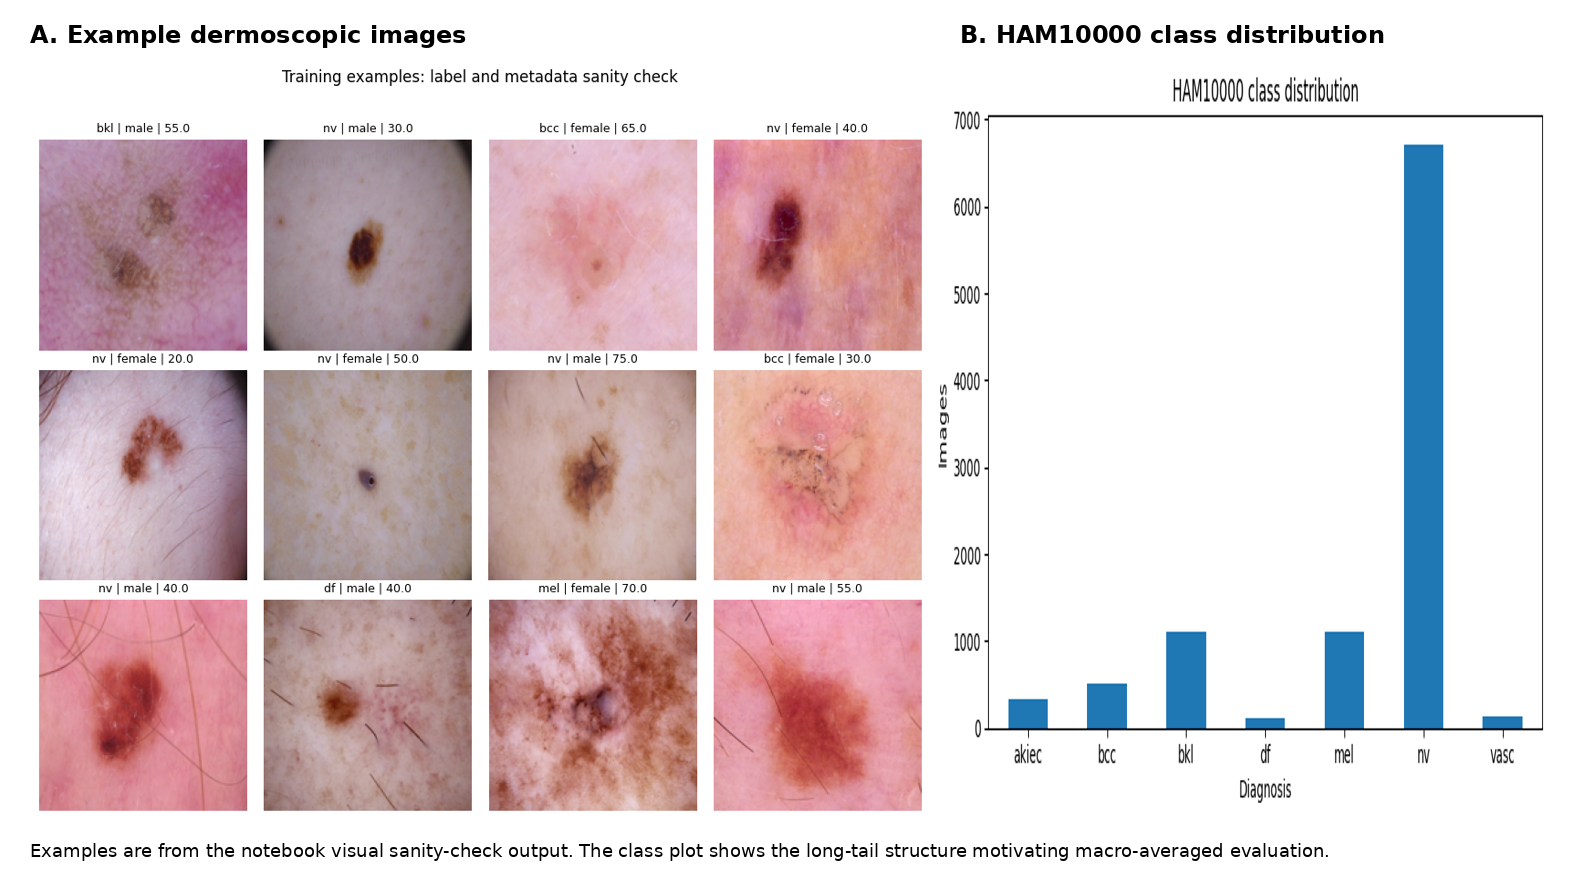
\includegraphics[width=0.98\textwidth]{fig_intro_overview.png}
\caption{Dataset overview. Panel A shows representative dermoscopic images extracted from the notebook visual sanity-check output. Panel B shows the HAM10000 class distribution, highlighting the dominance of melanocytic naevi and the rarity of dermatofibroma, vascular lesions, and actinic keratoses. The example images are included for visual context only and are not intended as stand-alone diagnostic evidence.}
\label{fig:intro_overview}
\end{figure*}

Evaluation is further complicated by class imbalance and probability uncertainty. HAM10000 is dominated by melanocytic naevi, while dermatofibroma, vascular lesions, and actinic keratoses are rare; consequently, accuracy can mask minority-class failure. Long-tail losses such as inverse-frequency weighting, focal loss, and effective-number class-balanced loss are plausible options, but their benefit is task-dependent and should be selected empirically using validation data \citep{buda2018imbalance,johnson2019imbalance,lin2017focal,cui2019classbalanced}. In addition, high AUROC or accuracy does not guarantee that predicted probabilities are clinically meaningful. Modern neural networks may be miscalibrated, and temperature scaling provides a simple validation-fitted post-hoc method for improving probability quality without changing the predicted class \citep{guo2017calibration,carse2022calibration,lambert2024uq}.

For clinical decision support, uncertainty should affect action. Selective classification formalises the trade-off between coverage and risk: a model may classify high-confidence cases while abstaining on uncertain cases \citep{elyaniv2010selective,geifman2019selectivenet}. In skin-lesion diagnosis, this naturally corresponds to selective referral, where uncertain or unusual lesions are escalated for expert review rather than forced into automatic classification \citep{mobiny2019riskaware,fayyad2024conformal}. Subgroup analysis is also necessary, because a fixed referral rule may not behave consistently across age, sex, anatomical site, or acquisition context. However, HAM10000 lacks reliable skin-tone labels, so it cannot support definitive skin-tone fairness claims; such claims require datasets with explicit skin-tone or diverse clinical metadata \citep{groh2021fitzpatrick17k,daneshjou2022disparities,alipour2024skintype,groh2024decision}.

This study addresses the gap between high-performing benchmark classifiers and clinically usable decision-support systems. In line with the title \textit{When Should Skin-Lesion AI Stay Silent?}, we ask whether a lesion-level, validation-selected HAM10000 classifier can support calibrated and selective decision-making rather than full-coverage prediction. Specifically, we evaluate balanced discrimination, temperature-scaled calibration, uncertainty-guided selective referral, subgroup reliability, external ISIC2018 robustness, stress-test behaviour, and computational feasibility. The objective is not to claim autonomous diagnosis, but to test whether a conventional transfer-learning classifier can identify a sufficiently reliable automatic subset while deferring higher-risk or less reliable cases for human review.

\section{Methods}

\subsection{Study design and reporting orientation}

This was a retrospective methodological evaluation using publicly available dermoscopic image datasets. The study was designed to evaluate skin-lesion AI as a calibrated decision-support workflow rather than as a leaderboard classifier. Training, validation, calibration, and final testing were separated; the final model was selected using validation macro-F1 only; and the held-out internal test set was reserved for final evaluation. The reporting logic was aligned with TRIPOD+AI and early-stage AI decision-support reporting principles, while recognising that this was not a prospective clinical trial or a deployed clinical evaluation \citep{collins2024tripodai,vasey2022decideai,liu2020consortai}.

\begin{figure}[H]
\centering
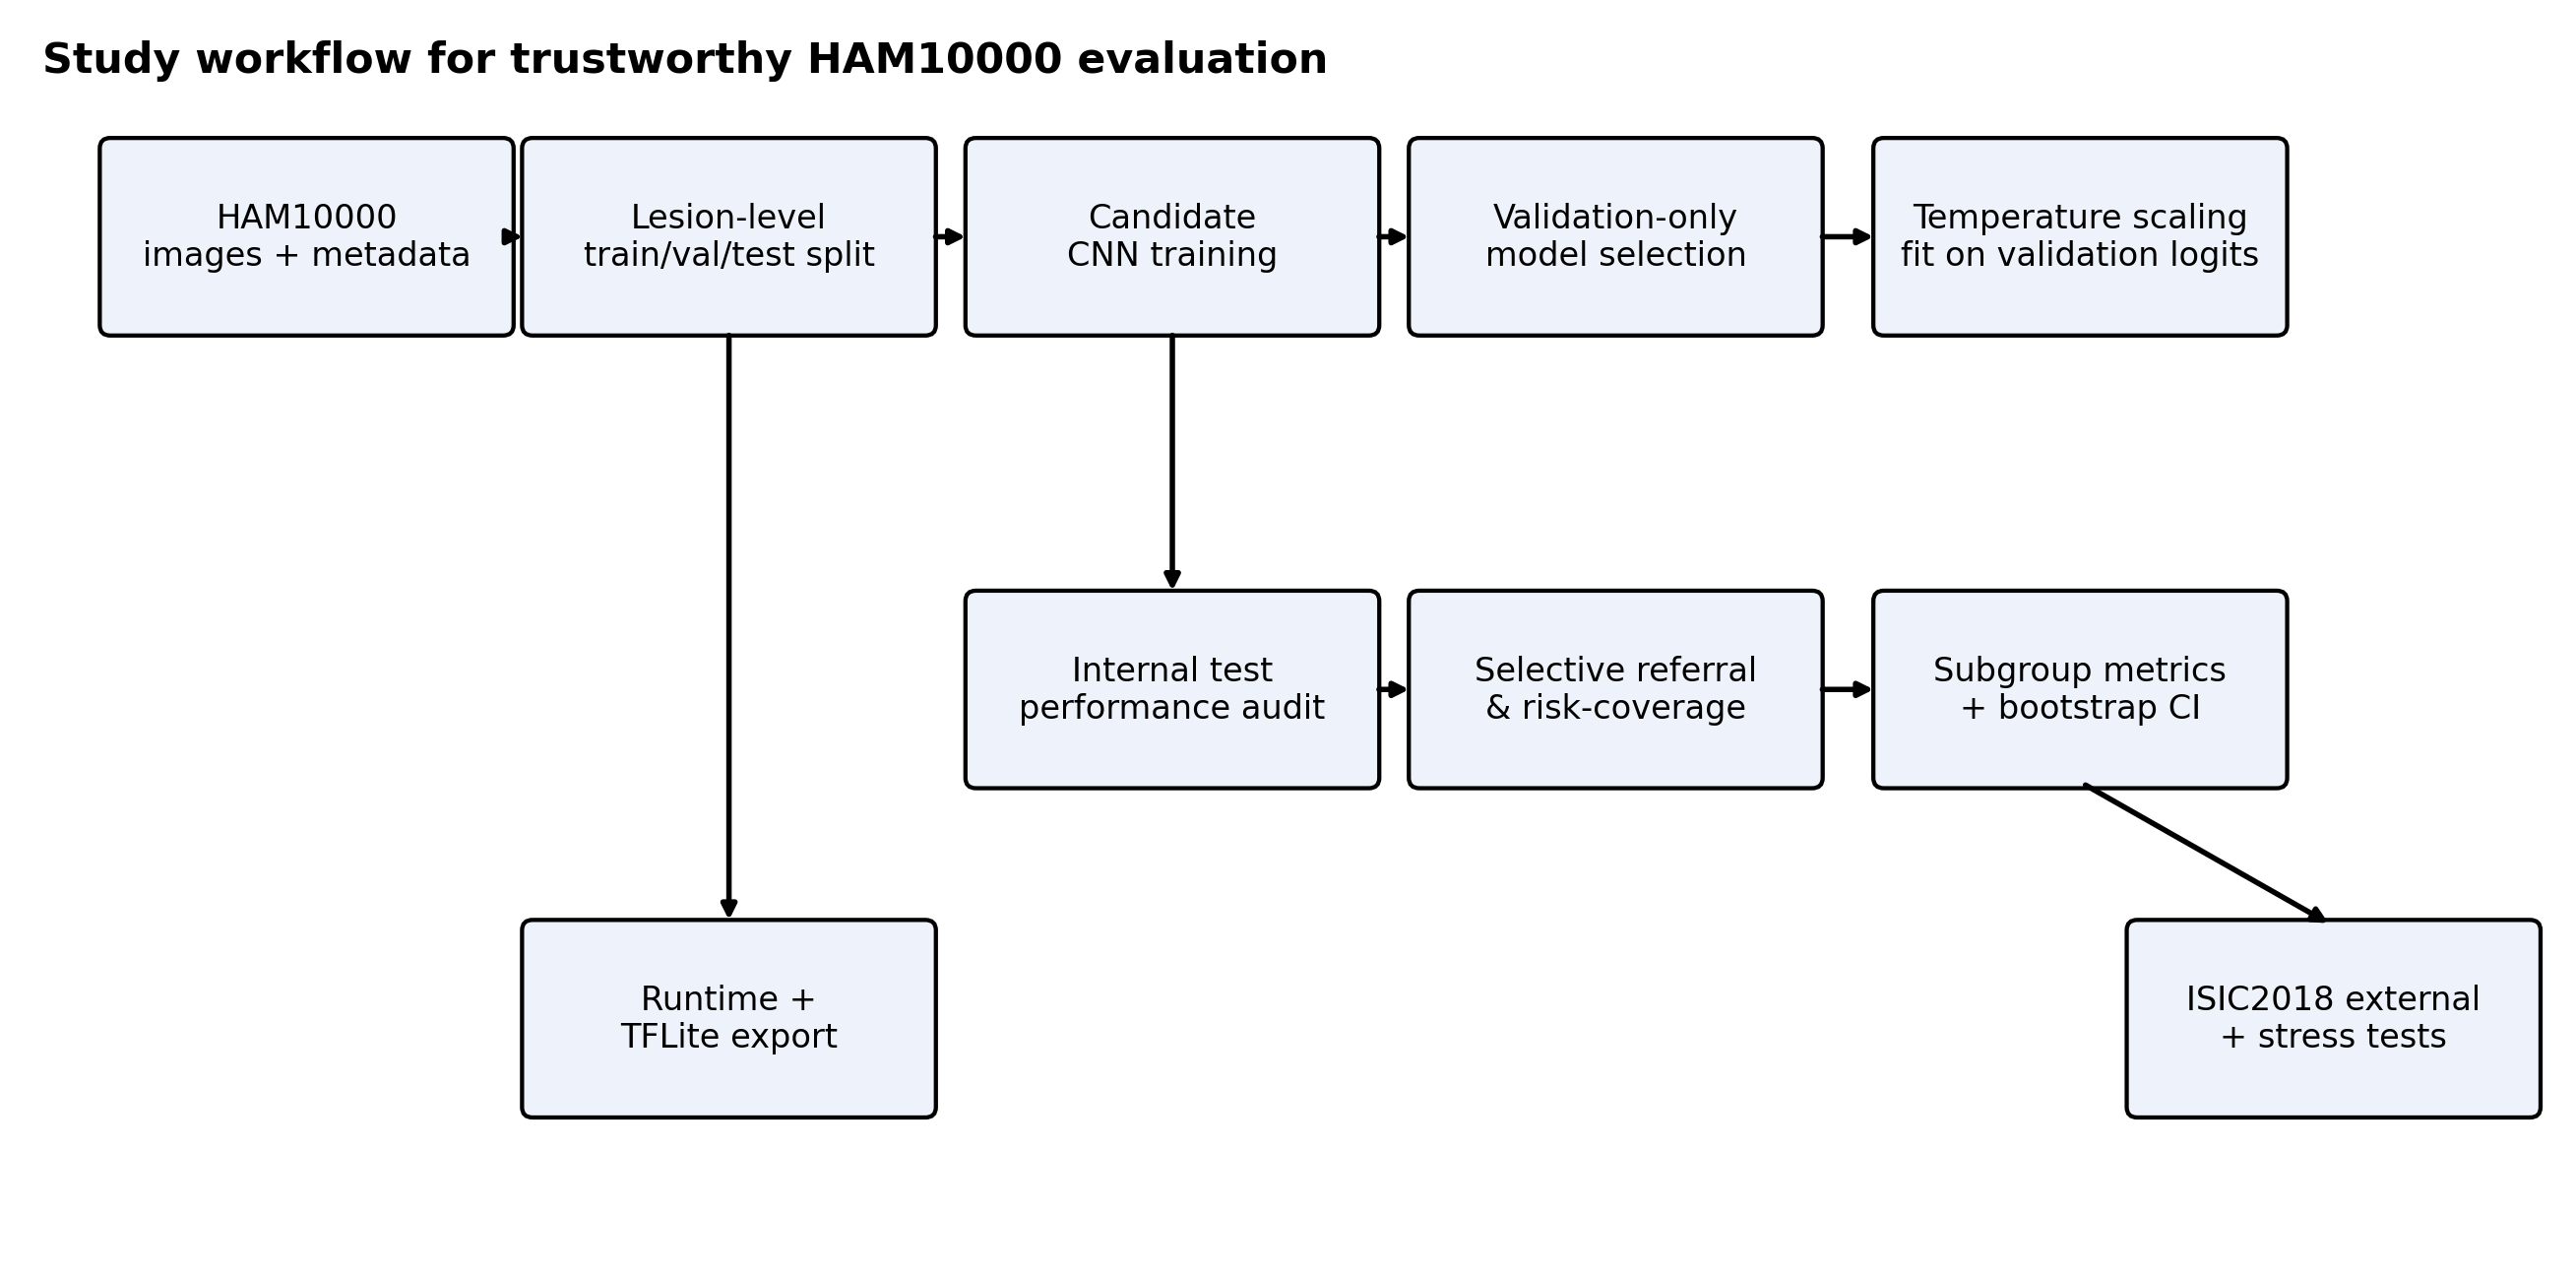
\includegraphics[width=0.98\linewidth]{fig_workflow.png}
\caption{Overview of the leakage-controlled, calibration-aware, and referral-oriented evaluation workflow. The pipeline starts with HAM10000 data auditing and lesion-level splitting, then proceeds through image-only candidate training, validation-only model selection, validation-fitted temperature scaling, internal test evaluation, selective-referral analysis, subgroup reliability assessment, external ISIC2018 testing, stress testing, and deployment-feasibility accounting.}
\label{fig:workflow}
\end{figure}

The central clinical question was whether the model could identify cases suitable for automatic classification while deferring less reliable cases for clinician review. The workflow therefore evaluates not only discrimination, but also probability calibration, uncertainty-guided referral, subgroup reliability, external robustness, and computational feasibility.

\subsection{Data sources}

The primary dataset was \dataset{}, consisting of 10,015 dermoscopic images from 7,470 unique lesions. The diagnosis labels were actinic keratoses and intraepithelial carcinoma (akiec), basal cell carcinoma (bcc), benign keratosis-like lesions (bkl), dermatofibroma (df), melanoma (mel), melanocytic naevi (nv), and vascular lesions (vasc). Dataset audit showed 1,956 lesions with multiple images, a maximum of six images per lesion, 57 missing ages, and 57 unknown sex entries. The class distribution was strongly imbalanced: nv accounted for 6,705 of 10,015 images (66.9\%), whereas df and vasc accounted for 115 (1.1\%) and 142 (1.4\%) images, respectively.

When available in the same archive, \isic{} Task 3 test data were used as a secondary external public benchmark. This external evaluation was interpreted as challenge-style out-of-sample testing within the dermoscopy ecosystem, not as evidence of real-world deployment performance \citep{codella2019isic2018,thomas2023deployment}.

\subsection{Lesion-level splitting and leakage control}

The data were split by \texttt{lesion\_id}. A first grouped split reserved approximately 20\% of the data for an independent internal test set. A second grouped split separated the remaining data into training and validation sets, producing 6,413 training images, 1,605 validation images, and 1,997 test images. There was no lesion identifier overlap between train, validation, and test sets. The train/validation/test class counts are shown in Table~\ref{tab:splits}. All preprocessing objects involving metadata were fitted only on the training set and then applied to validation, test, and external data.

\begin{table}[H]
\centering
\caption{Lesion-level split sizes and class counts.}
\label{tab:splits}
\begin{tabular}{lrrrrrrrr}
\toprule
Split & Total & akiec & bcc & bkl & df & mel & nv & vasc \\
\midrule
Train & 6413 & 203 & 329 & 681 & 69 & 695 & 4342 & 94 \\
Validation & 1605 & 56 & 100 & 192 & 18 & 199 & 1027 & 13 \\
Test & 1997 & 68 & 85 & 226 & 28 & 219 & 1336 & 35 \\
\bottomrule
\end{tabular}
\end{table}

\subsection{Image preprocessing and metadata policy}

Images were resized to $224\times224$ pixels and represented as RGB inputs. During training, conservative augmentation was applied using horizontal and vertical flips, light brightness and contrast perturbation, and mild central cropping. The augmentation policy was intended to improve robustness without destroying lesion-level visual semantics.

Metadata were handled conservatively. Age, sex, and anatomical site were considered deployable pre-diagnostic metadata and used only in a secondary clean late-fusion ablation. Diagnostic-confirmation type (\texttt{dx\_type}) was excluded from all model inputs because it encodes the pathway by which the diagnosis was confirmed, such as histology, follow-up, consensus, or confocal microscopy. It was retained only for subgroup analysis. This distinction prevents post-outcome or label-confirmation leakage and follows the principle that prediction inputs should be available at the intended time of prediction \citep{collins2024tripodai,hohn2021metadata}.

\subsection{Models and training}

Candidate image-only models used ImageNet-pretrained backbones from Keras Applications: EfficientNetB0, MobileNetV2, and ResNet50 \citep{he2016resnet,tan2019efficientnet,howard2017mobilenets,keras2024applications}. Each model used a global-average-pooled image embedding, dropout, a dense classification head, batch normalisation, and a seven-class logits output. Training used a two-stage transfer-learning procedure: a frozen-backbone head-training phase followed by low-learning-rate fine-tuning of the final backbone layers. The default batch size was 8, image size 224, dropout rate 0.30, head learning rate $10^{-3}$, fine-tuning learning rate $10^{-5}$, and early-stopping patience 5.

Long-tail handling was compared using three losses: inverse-frequency weighted cross-entropy, focal loss with $\gamma=2.0$, and effective-number class-balanced cross-entropy with $\beta=0.9999$ \citep{lin2017focal,cui2019classbalanced}. Inverse-frequency class weights in the training split were 4.513 for akiec, 2.785 for bcc, 1.345 for bkl, 13.277 for df, 1.318 for mel, 0.211 for nv, and 9.746 for vasc.

\subsection{Model selection and performance metrics}

The primary model was selected from the image-only candidate pool using validation macro-F1. Validation balanced accuracy, Brier score, expected calibration error (ECE), and one-vs-rest AUROC were retained as secondary selection and audit metrics. The test set was not used for architecture selection, loss selection, hyperparameter tuning, or temperature fitting.

Final metrics included accuracy, balanced accuracy, macro-F1, weighted-F1, macro recall, multiclass Brier score, negative log-likelihood (NLL), 15-bin ECE, and macro one-vs-rest ROC AUC. Per-class precision, recall, and F1 were also reported.

\subsection{Temperature scaling}

Temperature scaling was fitted on validation logits by optimising a scalar temperature $T$ to minimise validation NLL \citep{guo2017calibration}. The fitted value was $T=1.167$ with validation NLL 0.691. The same temperature was then applied to the internal test logits and external \isic{} logits. Since scalar temperature scaling preserves the ordering of logits, it was expected to affect probability quality without altering top-1 class predictions.

\subsection{Selective referral and uncertainty scores}

Selective referral was evaluated using three post-hoc uncertainty scores: maximum-probability uncertainty ($1-\max_k p_k$), predictive entropy, and negative margin between the two highest class probabilities. Samples were ordered from most certain to least certain. For target coverage levels of 95\%, 90\%, 80\%, 70\%, and 50\%, we reported achieved coverage, referral rate, selective risk, balanced accuracy and macro-F1 among automatically classified cases, and melanoma auto-detection among true melanoma cases. Area under the risk-coverage curve (AURC) was used as an aggregate summary \citep{elyaniv2010selective,geifman2019selectivenet}. MC Dropout was implemented as a computationally more expensive sensitivity analysis using repeated stochastic forward passes with dropout active \citep{gal2016dropout,lakshminarayanan2017ensembles}.

\subsection{Subgroup analysis and bootstrap uncertainty}

Internal subgroup reliability was assessed for sex, age bin, anatomical site, and diagnostic-confirmation type. Age was grouped into $\leq30$, 31--45, 46--60, 61--75, and $>75$ years. For each subgroup, we computed the same discrimination and calibration metrics and counted key minority/high-risk classes, especially mel, akiec, df, and vasc. Subgroup analyses were interpreted as metadata-defined reliability analyses, not as skin-tone fairness analyses, because \dataset{} lacks reliable skin-tone labels. Overall and subgroup uncertainty intervals were estimated using 1,000 bootstrap resamples. Subgroup bootstrap was run only when subgroup size was at least 30.

\subsection{External evaluation, stress tests, and deployment attempt}

External \isic{} evaluation used the validation-fitted \dataset{} temperature; the external labels were not used to re-fit calibration. Stress tests applied simple image perturbations, including brightness changes, contrast changes, JPEG compression, and central crop perturbation, to assess clinic-readiness sensitivity \citep{young2021stress,ovadia2019uncertainty}. Deployment feasibility was evaluated through runtime logs, methodological checks, and TensorFlow Lite export. The exported artifact is reported as a feasibility result rather than evidence of clinical deployment \citep{tensorflow2024tflite,thomas2023deployment}.



ewcommand{estmodel}{ResNet50 image-only weighted cross-entropy}

ewcommand{	flitesize}{24.455 MB}

\section{Results}

\subsection{Data audit}

The full \dataset{} table contained 10,015 image rows, 10,015 unique image identifiers, and 7,470 unique lesion identifiers. There were no duplicate image identifiers, but 1,956 lesions had multiple images, confirming the need for lesion-level splitting. Class imbalance was substantial: nv represented 66.9\% of the data, while df and vasc represented only 1.1\% and 1.4\%, respectively.

\subsection{Validation-based model selection}

Seven primary image-only candidates were evaluated on the validation split. The selected model was ResNet50 trained with inverse-frequency weighted cross-entropy, which achieved the highest validation macro-F1 (0.601) and validation balanced accuracy (0.695) within the prespecified primary candidate pool (Figure~\ref{fig:model_selection}). The ranking varied across architectures, losses, and random seeds, supporting empirical validation-based selection rather than assuming that a particular architecture or long-tail loss would dominate a priori \citep{gessert2020efficientnets,lin2017focal,cui2019classbalanced}.

\begin{figure}[H]
\centering
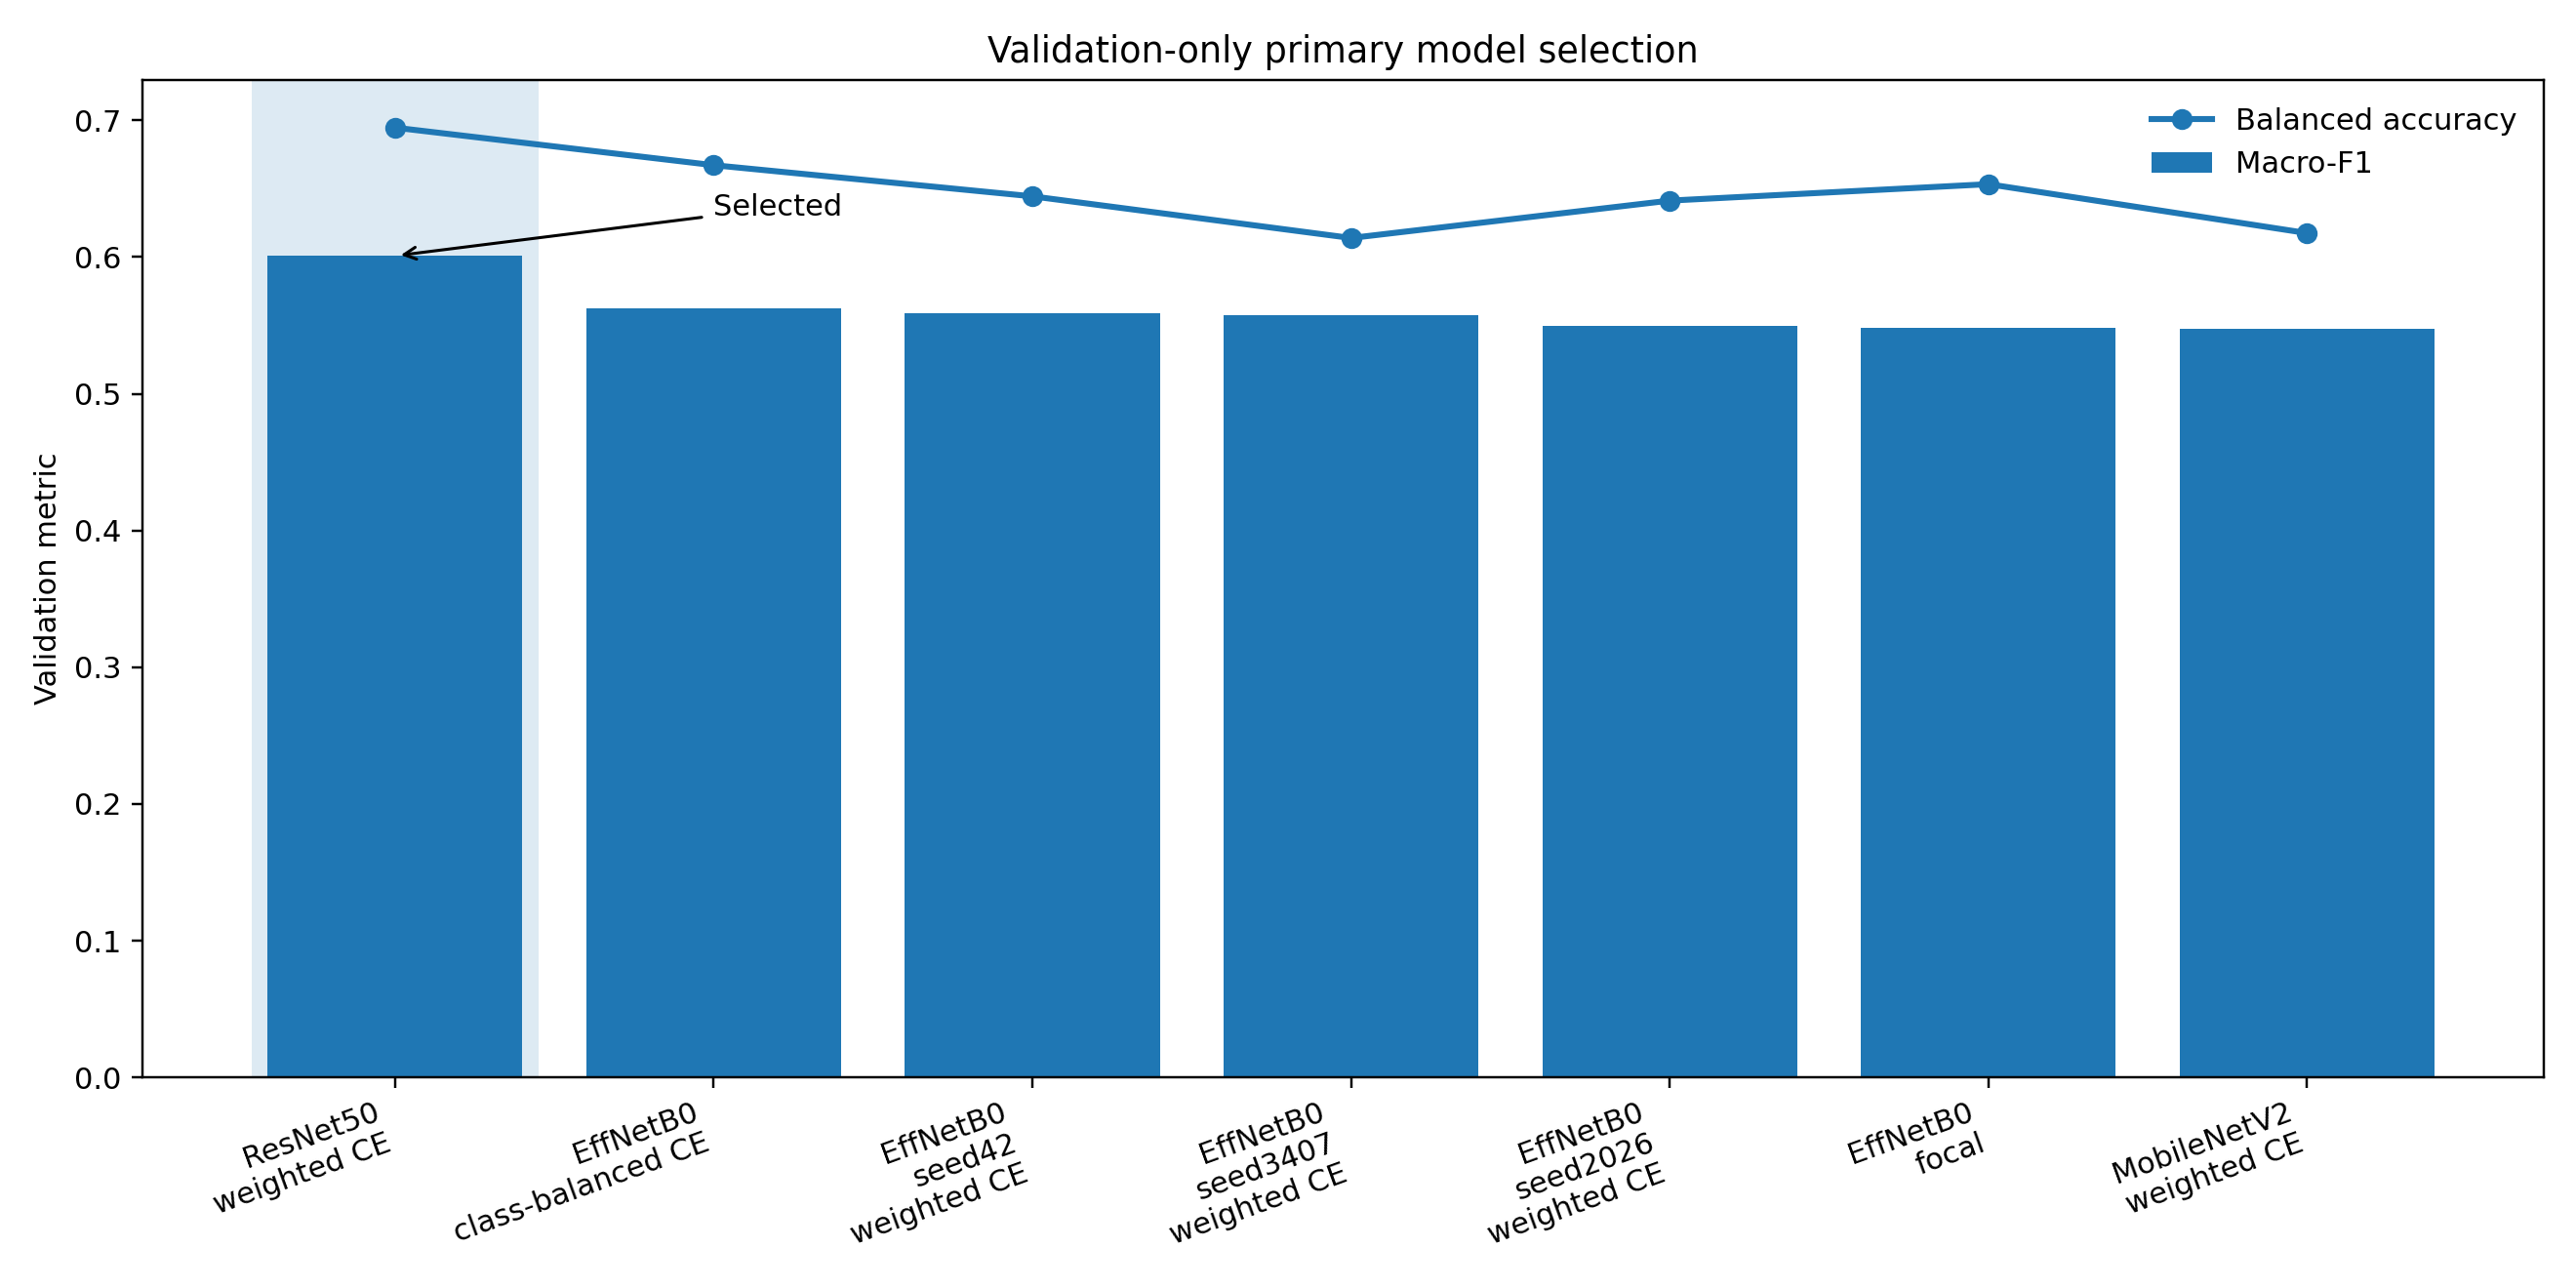
\includegraphics[width=0.98\linewidth]{fig_model_selection.png}
\caption{Validation-only primary model selection among image-only candidates. Bars show validation macro-F1, and the line shows validation balanced accuracy. The shaded first column indicates the validation-selected model used for locked internal test evaluation.}
\label{fig:model_selection}
\end{figure}

\subsection{Internal test performance and calibration}

On the independent internal test set, the selected ResNet50 model achieved accuracy 0.716, balanced accuracy 0.676, macro-F1 0.611, weighted-F1 0.740, and macro one-vs-rest AUROC 0.940 before calibration. Temperature scaling did not change top-1 predictions, but it improved probability quality: Brier score decreased from 0.381 to 0.376, NLL from 0.723 to 0.711, and ECE from 0.058 to 0.036 (Table~\ref{tab:test_calibration}; Figure~\ref{fig:calibration}). This indicates improved confidence calibration rather than improved class separation.

\begin{table}[H]
\centering
\caption{Internal test performance before and after temperature scaling.}
\label{tab:test_calibration}
\begin{tabular}{lrr}
\toprule
Metric & Raw & Temperature-scaled \\
\midrule
Accuracy & 0.716 & 0.716 \\
Balanced accuracy & 0.676 & 0.676 \\
Macro-F1 & 0.611 & 0.611 \\
Weighted-F1 & 0.740 & 0.740 \\
Macro recall & 0.676 & 0.676 \\
Brier score & 0.381 & 0.376 \\
NLL & 0.723 & 0.711 \\
ECE & 0.058 & 0.036 \\
Macro OVR ROC AUC & 0.940 & 0.940 \\
\bottomrule
\end{tabular}
\end{table}

\begin{figure}[H]
\centering
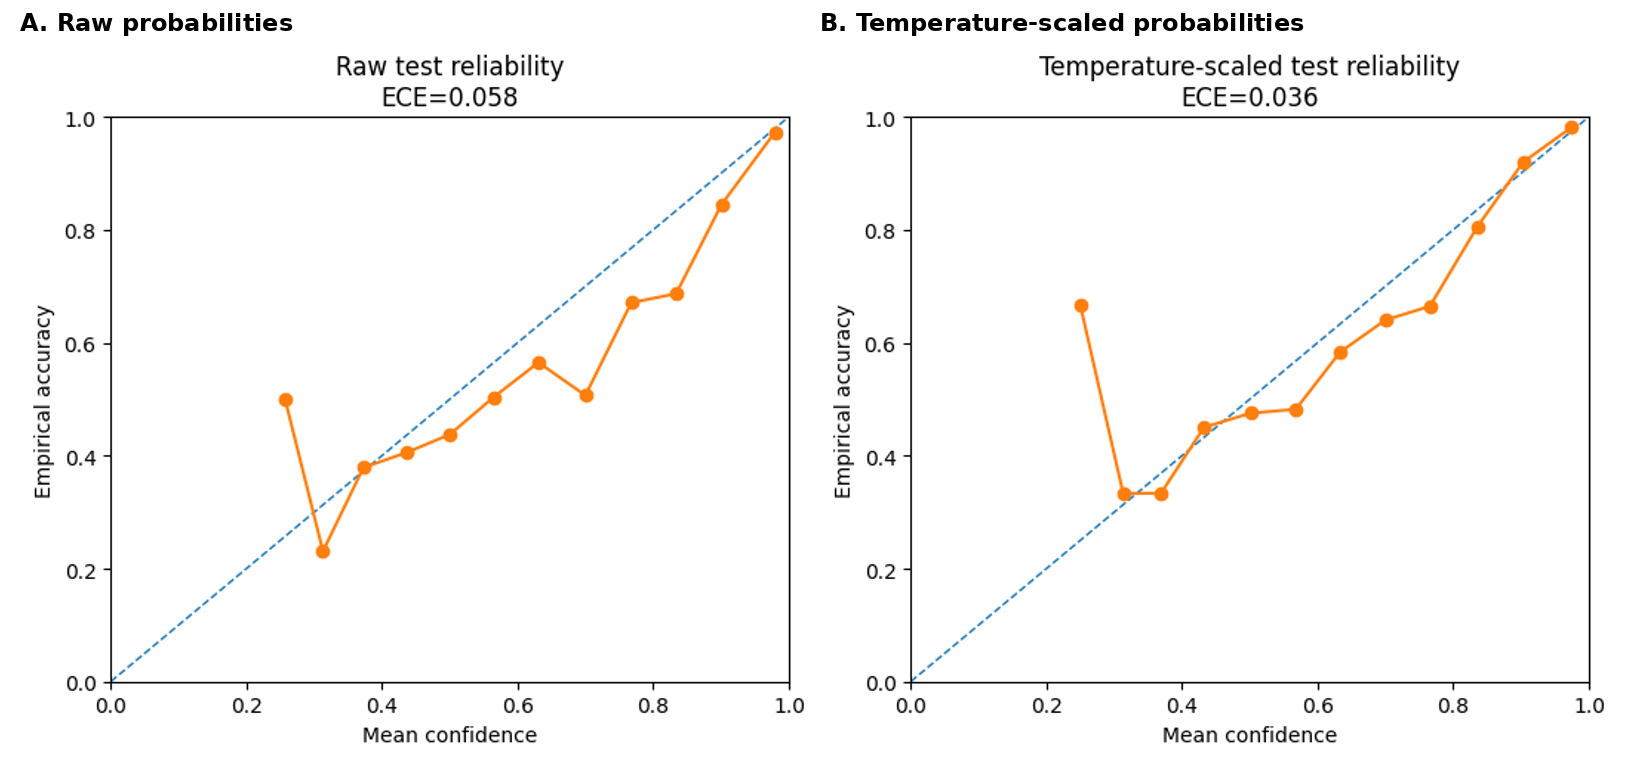
\includegraphics[width=0.98\linewidth]{fig_calibration_reliability.png}
\caption{Internal test-set reliability diagrams before and after temperature scaling. Calibration improved from ECE 0.058 to 0.036 without changing top-1 predictions.}
\label{fig:calibration}
\end{figure}

Per-class results showed why aggregate accuracy was insufficient. Melanoma recall was 0.626 but precision was 0.348, yielding F1 0.447. Dermatofibroma had recall 0.536 and F1 0.517. Vascular lesions had high recall (0.971) but moderate precision (0.630). Bootstrap uncertainty intervals after temperature scaling were 0.696--0.737 for accuracy, 0.640--0.715 for balanced accuracy, 0.573--0.648 for macro-F1, and 0.027--0.056 for ECE (Table~\ref{tab:bootstrap}).

\begin{table}[H]
\centering
\caption{Per-class internal test metrics for the selected model.}
\label{tab:per_class}
\begin{tabular}{lrrrr}
\toprule
Class & Support & Recall & Precision & F1 \\
\midrule
akiec & 68 & 0.500 & 0.680 & 0.576 \\
bcc & 85 & 0.624 & 0.457 & 0.527 \\
bkl & 226 & 0.735 & 0.517 & 0.607 \\
df & 28 & 0.536 & 0.500 & 0.517 \\
mel & 219 & 0.626 & 0.348 & 0.447 \\
nv & 1336 & 0.742 & 0.960 & 0.837 \\
vasc & 35 & 0.971 & 0.630 & 0.764 \\
\bottomrule
\end{tabular}
\end{table}

\begin{table}[H]
\centering
\caption{Bootstrap uncertainty intervals for internal test metrics after temperature scaling.}
\label{tab:bootstrap}
\begin{tabular}{lrrr}
\toprule
Metric & Bootstrap mean & Lower 95\% & Upper 95\% \\
\midrule
Accuracy & 0.717 & 0.696 & 0.737 \\
Balanced accuracy & 0.677 & 0.640 & 0.715 \\
Macro-F1 & 0.610 & 0.573 & 0.648 \\
Weighted-F1 & 0.741 & 0.723 & 0.758 \\
Brier score & 0.375 & 0.355 & 0.396 \\
NLL & 0.711 & 0.670 & 0.750 \\
ECE & 0.041 & 0.027 & 0.056 \\
Macro OVR ROC AUC & 0.941 & 0.929 & 0.949 \\
\bottomrule
\end{tabular}
\end{table}

\subsection{Selective referral}

Selective referral reduced error risk among automatically classified cases as coverage decreased. With maximum-probability uncertainty, selective risk decreased from 0.264 at 95\% coverage to 0.210 at 80\%, 0.169 at 70\%, and 0.084 at 50\%. Macro-F1 among retained cases increased from 0.631 at 95\% coverage to 0.668 at 80\%, 0.714 at 70\%, and 0.786 at 50\%. Entropy showed a similar pattern and achieved macro-F1 0.702 at 80\% coverage and 0.723 at 70\% coverage (Figure~\ref{fig:selective_referral}; Table~\ref{tab:selective}).

\begin{figure}[H]
\centering
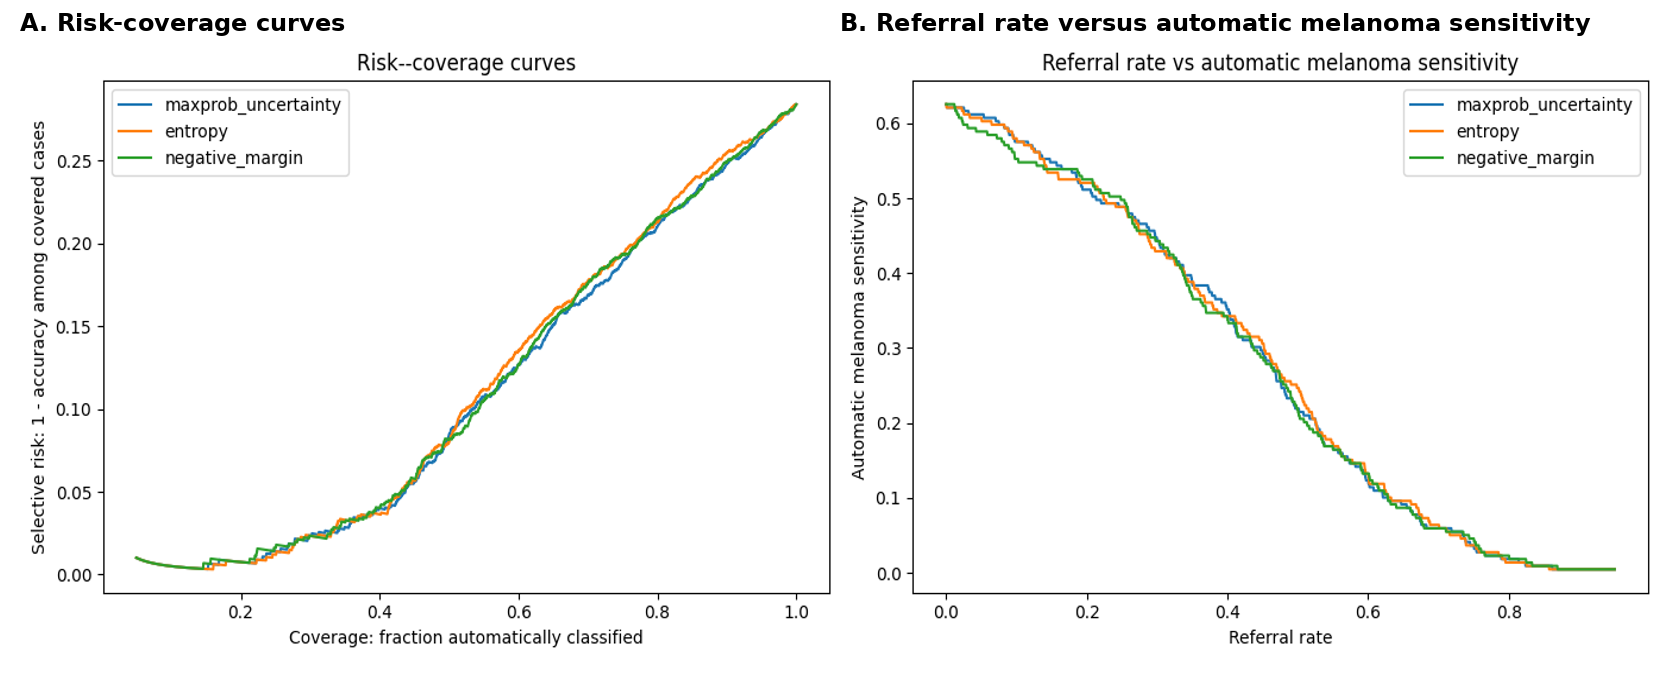
\includegraphics[width=0.98\linewidth]{fig_selective_referral.png}
\caption{Selective-referral behaviour on the internal test set. Panel A shows full risk-coverage curves for three uncertainty scores. Panel B shows the trade-off between referral rate and automatic melanoma sensitivity.}
\label{fig:selective_referral}
\end{figure}

\begin{table}[H]
\centering
\caption{Selective-referral operating points on the internal test set.}
\label{tab:selective}
\begin{tabular}{llrrrrr}
\toprule
Score & Coverage & Referral rate & Selective risk & BA & Macro-F1 & Mel auto recall \\
\midrule
Max-probability & 0.95 & 0.050 & 0.264 & 0.691 & 0.631 & 0.612 \\
Max-probability & 0.90 & 0.100 & 0.248 & 0.694 & 0.639 & 0.575 \\
Max-probability & 0.80 & 0.200 & 0.210 & 0.715 & 0.668 & 0.511 \\
Max-probability & 0.70 & 0.300 & 0.169 & 0.763 & 0.714 & 0.443 \\
Max-probability & 0.50 & 0.500 & 0.084 & 0.805 & 0.786 & 0.219 \\
Entropy & 0.80 & 0.200 & 0.213 & 0.749 & 0.702 & 0.521 \\
Entropy & 0.70 & 0.300 & 0.177 & 0.768 & 0.723 & 0.429 \\
Negative margin & 0.80 & 0.200 & 0.215 & 0.713 & 0.666 & 0.525 \\
\bottomrule
\end{tabular}
\end{table}

The melanoma auto-recall column is the fraction of all true melanoma cases both retained within the automatic-coverage subset and classified as melanoma. It can therefore decrease as coverage decreases even while selective risk improves. Clinically, this represents a safety-workload trade-off: referral improves the average reliability of automatic decisions but shifts a larger fraction of true melanoma cases into the referred group.

\subsection{Subgroup reliability}

Subgroup analysis showed clinically relevant heterogeneity (Figure~\ref{fig:subgroup_heatmaps}). Female-labelled cases had higher balanced accuracy (0.739 vs. 0.627), higher macro-F1 (0.664 vs. 0.566), lower Brier score (0.333 vs. 0.412), and lower ECE (0.018 vs. 0.066) than male-labelled cases. Younger cases aged $\leq30$ had low macro-F1 (0.356) despite moderate accuracy, while the 31--45 group had macro-F1 0.589. Anatomical-site and diagnostic-confirmation strata showed larger apparent variation, but these estimates were affected by class composition and small rare-class denominators \citep{groh2021fitzpatrick17k,daneshjou2022disparities,alipour2024skintype}.

\begin{figure}[H]
\centering
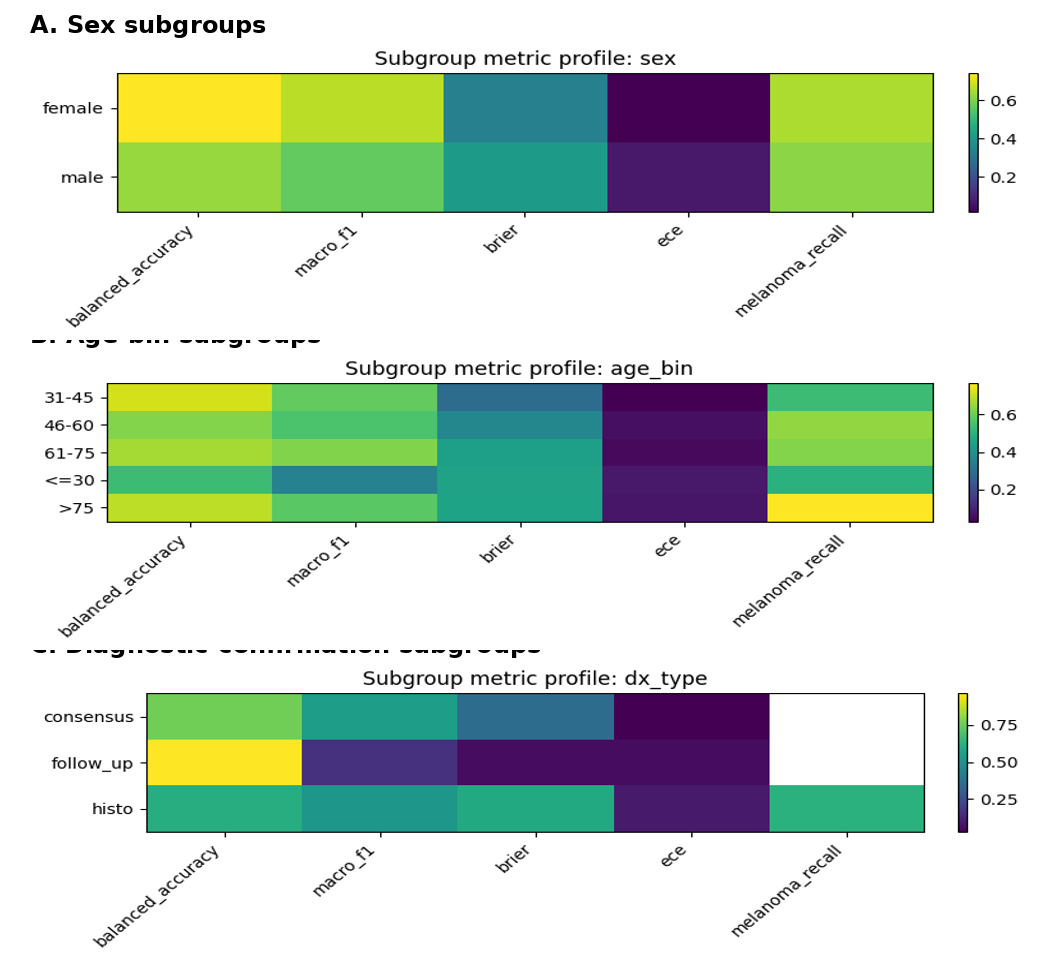
\includegraphics[width=0.86\linewidth]{fig_subgroup_heatmaps.png}
\caption{Subgroup reliability heatmaps after temperature scaling. Panels show balanced accuracy, macro-F1, Brier score, ECE, and melanoma recall across metadata-defined subgroup families. These are internal reliability analyses, not definitive skin-tone fairness estimates.}
\label{fig:subgroup_heatmaps}
\end{figure}

The subgroup gap summary confirmed a sex gap of 0.112 in balanced accuracy, 0.098 in macro-F1, and 0.048 in ECE. Age-bin gaps were 0.184 for balanced accuracy and 0.270 for macro-F1. Localization gaps were larger, reaching 0.531 for balanced accuracy and 0.415 for macro-F1. Melanoma recall ranged from 0 to 1 across localization groups, but this extreme range was driven by small subgroup denominators and should be interpreted as instability rather than a precise site-specific fairness estimate.

\subsection{External evaluation, stress testing, and deployment feasibility}

External \isic{} evaluation showed moderate transferability within the dermoscopy ecosystem: accuracy 0.698, balanced accuracy 0.635, macro-F1 0.608, ECE 0.038, and macro one-vs-rest AUROC 0.934. These results support related-domain robustness but not autonomous clinical readiness. Figure~\ref{fig:isic_external} shows the external confusion matrix and reliability diagram.

\begin{figure}[H]
\centering
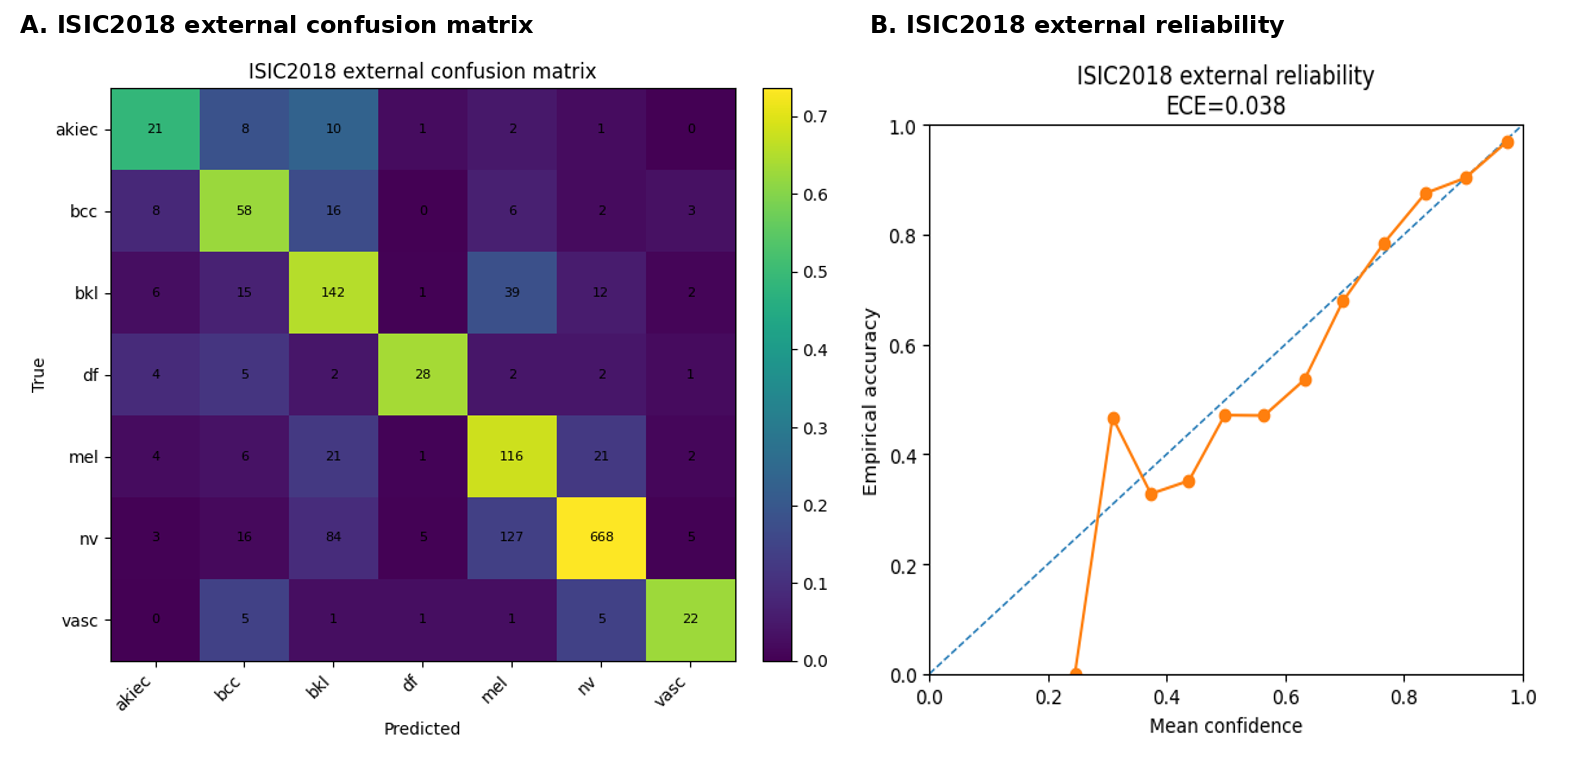
\includegraphics[width=0.98\linewidth]{fig_isic2018_external.png}
\caption{External ISIC2018 evaluation. Panel A shows the external confusion matrix. Panel B shows the external reliability diagram after applying the validation-fitted HAM10000 temperature.}
\label{fig:isic_external}
\end{figure}

Stress testing showed that aggregate accuracy could be misleading under perturbation. In a 1,000-image stress subset, JPEG quality 40 increased accuracy to 0.740 but reduced balanced accuracy to 0.620 and macro-F1 to 0.565. Brightness-down and contrast-up perturbations also reduced macro-F1, and contrast-up worsened ECE to 0.076. These results support reporting robustness beyond unperturbed aggregate accuracy \citep{young2021stress,ovadia2019uncertainty}.

Deployment feasibility was mixed. CPU-only training was feasible but costly: the selected ResNet50 required 8,017 seconds in total, including 3,123 seconds for head training and 4,894 seconds for fine-tuning. A TensorFlow Lite image-only export succeeded as a dynamic-range quantized model of 24.455 MB, and methodological verification confirmed that \texttt{dx\_type} was excluded from predictive metadata and that selective sensitivities were bounded by 1. This is deployment-feasibility evidence, not evidence of clinical deployment.

\section{Discussion}

\subsection{Interpretive summary}

This study asked when skin-lesion AI should remain silent rather than provide a full-coverage automatic diagnosis. The results suggest that the validation-selected ResNet50 is best understood as a calibrated triage-support candidate, not as an autonomous diagnostic system. Its main value is not clinically definitive discrimination, but the ability to organise outputs into a more clinically meaningful workflow: calibrated probabilities, selective referral of uncertain cases, subgroup reliability auditing, and external robustness checks \citep{guo2017calibration,elyaniv2010selective,collins2024tripodai,vasey2022decideai}.

The central interpretation is that a conventional dermoscopic classifier becomes more clinically interpretable when evaluated as a system that may defer. In this framing, the question is not only whether the model assigns the correct label, but whether it can identify predictions reliable enough for automatic support while keeping uncertain cases under human review.

\subsection{Model selection, calibration, and referral}

The selected ResNet50 should be interpreted as a locked validation-selected benchmark for reliability assessment, not as evidence that ResNet50 is universally superior for dermatology AI. Validation macro-F1 was appropriate because \dataset{} is a long-tailed seven-class task where accuracy can be dominated by melanocytic naevi. The finding that weighted cross-entropy outperformed focal loss and class-balanced loss reinforces that imbalance methods should be compared empirically rather than assumed to improve performance \citep{tschandl2018ham10000,lin2017focal,cui2019classbalanced,gessert2020efficientnets}.

Calibration was clinically important because temperature scaling improved Brier score, NLL, and ECE without changing top-1 predictions. This improved the trustworthiness of probability estimates, not the classifier's ranking ability. In a triage setting, probability quality is essential because referral rules and uncertainty flags depend on whether confidence values are meaningful \citep{guo2017calibration,carse2022calibration,lambert2024uq}.

Selective referral provides the practical answer to the title question. The model should stay silent when uncertainty is high enough that automatic classification would be unsafe. Lower automatic coverage reduced selective risk and improved macro-F1 among retained cases, supporting uncertainty-guided referral as a safer alternative to forced full-coverage classification \citep{elyaniv2010selective,geifman2019selectivenet,mobiny2019riskaware}. This remains a retrospective triage simulation, not a deployment-ready threshold. A real operating point would need to balance missed-melanoma risk, dermatology capacity, referral burden, patient safety priorities, and local workflow constraints \citep{thomas2023deployment,krakowski2024humanai}.

\subsection{Subgroup reliability and fairness boundaries}

Subgroup analyses showed that aggregate performance did not fully describe model behaviour. Reliability varied across sex, age, anatomical site, and diagnostic-confirmation strata, indicating that a model can appear acceptable on average while remaining less reliable for specific groups or lesion contexts. These results should be reported with denominators and bootstrap uncertainty, especially when rare classes are sparse within subgroups \citep{collins2024tripodai,daneshjou2022disparities,alipour2024skintype}.

These findings are not a complete fairness audit. \dataset{} does not provide reliable skin-tone labels, so this study cannot establish fairness across skin tones. The appropriate claim is narrower: the model shows internal reliability heterogeneity across available metadata-defined strata. Future fairness evaluation should use datasets with explicit skin-tone or diverse clinical metadata, such as Fitzpatrick17k, DDI, PAD-UFES-20, or MIDAS \citep{groh2021fitzpatrick17k,daneshjou2022disparities,pacheco2020padufes,chiou2025midas}. Diagnostic-confirmation type is useful for post-hoc subgroup interpretation, but should not be used as a predictive input because it encodes a downstream confirmation pathway rather than a pre-diagnostic feature \citep{tschandl2018ham10000,collins2024tripodai}.

\subsection{Contribution and clinical implications}

This study does not claim architectural novelty. CNNs and EfficientNet-style models have already shown meaningful performance on \dataset{} and ISIC-style benchmarks \citep{tschandl2018ham10000,codella2019isic2018,gessert2020efficientnets}. The contribution is evaluative: lesion-level leakage control, validation-only model selection, calibration, selective referral, subgroup reliability, external testing, stress testing, and deployment-feasibility reporting are linked into a single clinically oriented assessment chain \citep{cassidy2022isic,young2021stress,ovadia2019uncertainty}.

Clinically, the model should be framed as an assistive triage candidate, not an autonomous diagnostic device. Its calibrated probabilities and uncertainty scores may support prioritisation or second-read workflows, but its moderate macro-F1, subgroup heterogeneity, and retrospective-only validation make full automation inappropriate. Uncertain, unusual, or high-risk cases should remain under human oversight \citep{vasey2022decideai,thomas2023deployment,krakowski2024humanai}. Methodologically, future skin-lesion AI studies should report more than accuracy or AUROC, including leakage-controlled splitting, validation-only model selection, calibration, subgroup denominators, uncertainty-guided referral behaviour, external testing, stress testing, and deployment constraints \citep{collins2024tripodai,cassidy2022isic,young2021stress,tensorflow2024tflite}.

\section{Limitations}

Several limitations bound the strength of these conclusions. First, this was a retrospective public-dataset study. \dataset{} and \isic{} are valuable benchmarks, but they do not capture prospective clinical workflows, changing acquisition devices, referral pathways, clinician behaviour, or population shifts. The external \isic{} analysis should therefore be interpreted as related-domain challenge-style testing, not as proof of real-world deployment readiness \citep{codella2019isic2018,thomas2023deployment}.

Second, subgroup analysis was limited by available metadata. Sex, age, anatomical site, and diagnostic-confirmation type were available, but reliable skin-tone labels were not. Some subgroup estimates were also unstable because rare classes had small denominators within certain strata. Future work should test the same framework on datasets with explicit skin-tone and rare-disease labels, and should report subgroup-specific coverage, referral burden, and melanoma handling \citep{groh2021fitzpatrick17k,daneshjou2022disparities,alipour2024skintype}.

Third, selective referral was evaluated retrospectively. The analysis showed that uncertainty-guided deferral can reduce selective risk among retained cases, but it did not test whether clinicians would use these referrals effectively or whether workflow-level outcomes would improve. Reader studies and early-stage clinical evaluations are needed before clinical deployment claims can be made \citep{krakowski2024humanai,vasey2022decideai}.

Fourth, uncertainty estimation and deployment evaluation were limited. Softmax-derived scores were used as the main referral signals, while MC Dropout was a computationally expensive sensitivity analysis. Future work should compare deep ensembles and conformal prediction methods \citep{lakshminarayanan2017ensembles,fayyad2024conformal,lu2022fairconformal}. Although TensorFlow Lite export succeeded, an actual deployment would still require numerical equivalence checks, latency and memory profiling, clinical governance, and post-deployment monitoring \citep{tensorflow2024tflite,thomas2023deployment}.
\section{Conclusion}

A skin-lesion AI model trained on \dataset{} can be evaluated more responsibly by combining lesion-level splitting, validation-only model selection, probability calibration, risk-coverage analysis, subgroup reliability assessment, external benchmark testing, and deployment-feasibility reporting. The validation-selected image-only ResNet50 achieved moderate discrimination and improved calibration after temperature scaling. Selective referral reduced error risk among automatically classified cases, but subgroup results showed important reliability heterogeneity. The model should therefore be considered a calibrated triage-support candidate, not an autonomous diagnostic system. Future work should extend this workflow to datasets with explicit skin-tone labels, multi-institutional clinical images, and prospective human-AI evaluation.

\section*{Data availability}

\dataset{} and \isic{} are publicly available benchmark datasets subject to their respective data-use terms. The processed split files and derived outputs should be released with the code repository where licensing permits. No new patient data were collected in this study.

\section*{Code availability}

The analysis was implemented in Python using TensorFlow/Keras, scikit-learn, NumPy, pandas, and Matplotlib. The reproducible notebook, model-selection tables, calibration outputs, subgroup summaries, risk-coverage outputs, and manifest files should be deposited at: \codeplaceholder{}.

\section*{Ethics statement}

This study used publicly available, de-identified image datasets and did not involve prospective recruitment, intervention, or access to identifiable patient records. Formal institutional review was not required for the analysis of these public benchmark data, subject to local institutional policy.

\section*{Author contributions}

T.Y. conceived the study, implemented the notebook workflow, conducted the analysis, interpreted the results, and drafted the manuscript.

\section*{Competing interests}

The author declares no competing interests.

\section*{Funding}

No specific funding was received for this study.

\section*{Acknowledgements}

The author acknowledges the creators and maintainers of the \dataset{} and ISIC benchmark resources, and the open-source scientific Python and TensorFlow/Keras communities.


\begin{thebibliography}{99}
\bibitem[Tschandl et~al.(2018)]{tschandl2018ham10000} Tschandl, P., Rosendahl, C., \& Kittler, H. (2018). The HAM10000 dataset, a large collection of multi-source dermatoscopic images of common pigmented skin lesions. \textit{Scientific Data}, 5, 180161. https://doi.org/10.1038/sdata.2018.161
\bibitem[Codella et~al.(2019)]{codella2019isic2018} Codella, N. C. F., Rotemberg, V., Tschandl, P., Celebi, M. E., Dusza, S., Gutman, D., et al. (2019). Skin lesion analysis toward melanoma detection 2018: A challenge hosted by the International Skin Imaging Collaboration. \textit{arXiv:1902.03368}. https://doi.org/10.48550/arXiv.1902.03368
\bibitem[Cassidy et~al.(2022)]{cassidy2022isic} Cassidy, B., Kendrick, C., Brodzicki, A., Jaworek-Korjakowska, J., \& Yap, M. H. (2022). Analysis of the ISIC image datasets: Usage, benchmarks and recommendations. \textit{Medical Image Analysis}, 75, 102305. https://doi.org/10.1016/j.media.2021.102305
\bibitem[Abhishek et~al.(2025)]{abhishek2025quality} Abhishek, K., Jain, A., \& Hamarneh, G. (2025). Investigating the quality of DermaMNIST and Fitzpatrick17k dermatological image datasets. \textit{Scientific Data}, 12, 196. https://doi.org/10.1038/s41597-025-04382-5
\bibitem[Esteva et~al.(2017)]{esteva2017dermatologist} Esteva, A., Kuprel, B., Novoa, R. A., Ko, J., Swetter, S. M., Blau, H. M., \& Thrun, S. (2017). Dermatologist-level classification of skin cancer with deep neural networks. \textit{Nature}, 542, 115-118. https://doi.org/10.1038/nature21056
\bibitem[Gessert et~al.(2020)]{gessert2020efficientnets} Gessert, N., Nielsen, M., Shaikh, M., Werner, R., \& Schlaefer, A. (2020). Skin lesion classification using ensembles of multi-resolution EfficientNets with meta data. \textit{MethodsX}, 7, 100864. https://doi.org/10.1016/j.mex.2020.100864
\bibitem[Hohn et~al.(2021)]{hohn2021metadata} Hohn, J., Hekler, A., Krieghoff-Henning, E., Kather, J. N., Utikal, J. S., \& Brinker, T. J. (2021). Integrating patient data into skin cancer classification using convolutional neural networks: Systematic review. \textit{Journal of Medical Internet Research}, 23(7), e20708. https://doi.org/10.2196/20708
\bibitem[Pacheco et~al.(2020)]{pacheco2020padufes} Pacheco, A. G. C., Lima, G. R., Salomao, A. S., Krohling, B., Biral, I. P., de Angelo, G. G., et al. (2020). PAD-UFES-20: A skin lesion dataset composed of patient data and clinical images collected from smartphones. \textit{Data in Brief}, 32, 106221. https://doi.org/10.1016/j.dib.2020.106221
\bibitem[Chiou et~al.(2025)]{chiou2025midas} Chiou, A. S., et al. (2025). Multimodal Image Dataset for AI-Based Skin Cancer Benchmarking (MIDAS). \textit{NEJM AI}. https://doi.org/10.1056/AIdbp2400732
\bibitem[He et~al.(2016)]{he2016resnet} He, K., Zhang, X., Ren, S., \& Sun, J. (2016). Deep residual learning for image recognition. \textit{Proceedings of the IEEE Conference on Computer Vision and Pattern Recognition}, 770-778. https://doi.org/10.1109/CVPR.2016.90
\bibitem[Tan and Le(2019)]{tan2019efficientnet} Tan, M., \& Le, Q. V. (2019). EfficientNet: Rethinking model scaling for convolutional neural networks. \textit{Proceedings of the 36th International Conference on Machine Learning}, PMLR 97, 6105-6114.
\bibitem[Howard et~al.(2017)]{howard2017mobilenets} Howard, A. G., Zhu, M., Chen, B., Kalenichenko, D., Wang, W., Weyand, T., et al. (2017). MobileNets: Efficient convolutional neural networks for mobile vision applications. \textit{arXiv:1704.04861}.
\bibitem[Buda et~al.(2018)]{buda2018imbalance} Buda, M., Maki, A., \& Mazurowski, M. A. (2018). A systematic study of the class imbalance problem in convolutional neural networks. \textit{Neural Networks}, 106, 249-259. https://doi.org/10.1016/j.neunet.2018.07.011
\bibitem[Johnson and Khoshgoftaar(2019)]{johnson2019imbalance} Johnson, J. M., \& Khoshgoftaar, T. M. (2019). Survey on deep learning with class imbalance. \textit{Journal of Big Data}, 6, 27. https://doi.org/10.1186/s40537-019-0192-5
\bibitem[Lin et~al.(2017)]{lin2017focal} Lin, T.-Y., Goyal, P., Girshick, R., He, K., \& Dollar, P. (2017). Focal loss for dense object detection. \textit{Proceedings of the IEEE International Conference on Computer Vision}, 2980-2988. https://doi.org/10.1109/ICCV.2017.324
\bibitem[Cui et~al.(2019)]{cui2019classbalanced} Cui, Y., Jia, M., Lin, T.-Y., Song, Y., \& Belongie, S. (2019). Class-balanced loss based on effective number of samples. \textit{Proceedings of the IEEE/CVF Conference on Computer Vision and Pattern Recognition}, 9268-9277.
\bibitem[Guo et~al.(2017)]{guo2017calibration} Guo, C., Pleiss, G., Sun, Y., \& Weinberger, K. Q. (2017). On calibration of modern neural networks. \textit{Proceedings of the 34th International Conference on Machine Learning}, PMLR 70, 1321-1330.
\bibitem[Carse et~al.(2022)]{carse2022calibration} Carse, J., Alvarez Olmo, A., \& McKenna, S. J. (2022). Calibration of deep medical image classifiers: An empirical comparison using dermatology and histopathology datasets. \textit{Uncertainty for Safe Utilization of Machine Learning in Medical Imaging}, LNCS, 89-99. https://doi.org/10.1007/978-3-031-16749-2\_9
\bibitem[Ovadia et~al.(2019)]{ovadia2019uncertainty} Ovadia, Y., Fertig, E., Ren, J., Nado, Z., Sculley, D., Nowozin, S., et al. (2019). Can you trust your model's uncertainty? Evaluating predictive uncertainty under dataset shift. \textit{Advances in Neural Information Processing Systems}, 32.
\bibitem[Lambert et~al.(2024)]{lambert2024uq} Lambert, B., Forbes, F., Tucholka, A., et al. (2024). Trustworthy clinical AI solutions: A unified review of uncertainty quantification in deep learning models for medical image analysis. \textit{Artificial Intelligence in Medicine}, 150, 102830. https://doi.org/10.1016/j.artmed.2024.102830
\bibitem[Gal and Ghahramani(2016)]{gal2016dropout} Gal, Y., \& Ghahramani, Z. (2016). Dropout as a Bayesian approximation: Representing model uncertainty in deep learning. \textit{Proceedings of the 33rd International Conference on Machine Learning}, PMLR 48, 1050-1059.
\bibitem[Lakshminarayanan et~al.(2017)]{lakshminarayanan2017ensembles} Lakshminarayanan, B., Pritzel, A., \& Blundell, C. (2017). Simple and scalable predictive uncertainty estimation using deep ensembles. \textit{Advances in Neural Information Processing Systems}, 30.
\bibitem[El-Yaniv and Wiener(2010)]{elyaniv2010selective} El-Yaniv, R., \& Wiener, Y. (2010). On the foundations of noise-free selective classification. \textit{Journal of Machine Learning Research}, 11, 1605-1641.
\bibitem[Geifman and El-Yaniv(2019)]{geifman2019selectivenet} Geifman, Y., \& El-Yaniv, R. (2019). SelectiveNet: A deep neural network with an integrated reject option. \textit{Proceedings of the 36th International Conference on Machine Learning}, PMLR 97, 2151-2159.
\bibitem[Geifman and El-Yaniv(2017)]{geifman2017selective} Geifman, Y., \& El-Yaniv, R. (2017). Selective classification for deep neural networks. \textit{Advances in Neural Information Processing Systems}, 30.
\bibitem[Mobiny et~al.(2019)]{mobiny2019riskaware} Mobiny, A., Singh, A., \& Nguyen, H. V. (2019). Risk-aware machine learning classifier for skin lesion diagnosis. \textit{Journal of Clinical Medicine}, 8(8), 1241. https://doi.org/10.3390/jcm8081241
\bibitem[Fayyad et~al.(2024)]{fayyad2024conformal} Fayyad, J., Alijani, S., \& Najjaran, H. (2024). Empirical validation of conformal prediction for trustworthy skin lesions classification. \textit{Computer Methods and Programs in Biomedicine}, 253, 108231. https://doi.org/10.1016/j.cmpb.2024.108231
\bibitem[Lu et~al.(2022)]{lu2022fairconformal} Lu, C., Lemay, A., Chang, K., Hobel, K., \& Kalpathy-Cramer, J. (2022). Fair conformal predictors for applications in medical imaging. \textit{Proceedings of the AAAI Conference on Artificial Intelligence}, 36(11), 12008-12016. https://doi.org/10.1609/aaai.v36i11.21459
\bibitem[Groh et~al.(2021)]{groh2021fitzpatrick17k} Groh, M., Harris, C., Soenksen, L., Lau, F., Han, R., Kim, A., Koochek, A., \& Badri, O. (2021). Evaluating deep neural networks trained on clinical images in dermatology with the Fitzpatrick 17k dataset. \textit{CVPR Workshop}.
\bibitem[Daneshjou et~al.(2022)]{daneshjou2022disparities} Daneshjou, R., Vodrahalli, K., Novoa, R. A., Jenkins, M., Liang, W., Rotemberg, V., et al. (2022). Disparities in dermatology AI performance on a diverse, curated clinical image set. \textit{Science Advances}, 8(32), eabq6147. https://doi.org/10.1126/sciadv.abq6147
\bibitem[Alipour et~al.(2024)]{alipour2024skintype} Alipour, N., Burke, T., \& Courtney, J. (2024). Skin type diversity in skin lesion datasets: A review. \textit{Current Dermatology Reports}, 13, 198-210. https://doi.org/10.1007/s13671-024-00440-0
\bibitem[Fogelberg et~al.(2023)]{fogelberg2023domain} Fogelberg, K., Chamarthi, S., Maron, R. C., Niebling, J., \& Brinker, T. J. (2023). Domain shifts in dermoscopic skin cancer datasets: Evaluation of essential limitations for clinical translation. \textit{New Biotechnology}. arXiv:2304.06968.
\bibitem[Young et~al.(2021)]{young2021stress} Young, A. T., Fernandez, K., Pfau, J., et al. (2021). Stress testing reveals gaps in clinic readiness of image-based diagnostic artificial intelligence models. \textit{npj Digital Medicine}, 4, 10. https://doi.org/10.1038/s41746-020-00380-6
\bibitem[Thomas et~al.(2023)]{thomas2023deployment} Thomas, L., Hyde, C., Mullarkey, D., et al. (2023). Real-world post-deployment performance of a novel machine learning-based digital health technology for skin lesion assessment and suggestions for post-market surveillance. \textit{Frontiers in Medicine}, 10, 1264846. https://doi.org/10.3389/fmed.2023.1264846
\bibitem[Krakowski et~al.(2024)]{krakowski2024humanai} Krakowski, I., Kim, J., Cai, Z. R., et al. (2024). Human-AI interaction in skin cancer diagnosis: A systematic review and meta-analysis. \textit{npj Digital Medicine}, 7, 78. https://doi.org/10.1038/s41746-024-01031-w
\bibitem[Groh et~al.(2024)]{groh2024decision} Groh, M., Badri, O., Daneshjou, R., et al. (2024). Deep learning-aided decision support for diagnosis of skin disease across skin tones. \textit{Nature Medicine}, 30, 573-583. https://doi.org/10.1038/s41591-023-02728-3
\bibitem[Selvaraju et~al.(2017)]{selvaraju2017gradcam} Selvaraju, R. R., Cogswell, M., Das, A., Vedantam, R., Parikh, D., \& Batra, D. (2017). Grad-CAM: Visual explanations from deep networks via gradient-based localization. \textit{Proceedings of the IEEE International Conference on Computer Vision}, 618-626. https://doi.org/10.1109/ICCV.2017.74
\bibitem[Giavina-Bianchi et~al.(2023)]{giavina2023xai} Giavina-Bianchi, M., Giavina-Bianchi, P., Santos, A. P., et al. (2023). Explainability agreement between dermatologists and five visual explanation techniques in deep neural networks for melanoma AI classification. \textit{Frontiers in Medicine}, 10, 1241484. https://doi.org/10.3389/fmed.2023.1241484
\bibitem[Collins et~al.(2024)]{collins2024tripodai} Collins, G. S., et al. (2024). TRIPOD+AI statement: Updated guidance for reporting clinical prediction models that use regression or machine learning methods. \textit{BMJ}, 385, e078378. https://doi.org/10.1136/bmj-2023-078378
\bibitem[Vasey et~al.(2022)]{vasey2022decideai} Vasey, B., Nagendran, M., Campbell, B., et al. (2022). Reporting guideline for the early-stage clinical evaluation of decision support systems driven by artificial intelligence: DECIDE-AI. \textit{Nature Medicine}, 28, 924-933. https://doi.org/10.1038/s41591-022-01772-9
\bibitem[Liu et~al.(2020)]{liu2020consortai} Liu, X., Rivera, S. C., Moher, D., Calvert, M. J., \& Denniston, A. K. (2020). Reporting guidelines for clinical trial reports for interventions involving artificial intelligence: The CONSORT-AI extension. \textit{BMJ}, 370, m3164. https://doi.org/10.1136/bmj.m3164
\bibitem[Keras Developers(2024)]{keras2024applications} Keras Developers. (2024). Keras Applications documentation. https://keras.io/api/applications/
\bibitem[TensorFlow Developers(2024)]{tensorflow2024tflite} TensorFlow Developers. (2024). tf.lite.TFLiteConverter API documentation. https://www.tensorflow.org/api\_docs/python/tf/lite/TFLiteConverter
\end{thebibliography}


\end{document}
